\documentclass{article}

\usepackage{lipsum}
\usepackage[margin=2cm, left=2cm, includefoot]{geometry}
\usepackage{graphicx}
\usepackage{float}
\usepackage{hyperref}

% Header and footer
\usepackage{fancyhdr}
\pagestyle{fancy}

\rhead{}
\lhead{}
\fancyfoot{}
\fancyfoot[R]{\thepage}
\renewcommand{\headrulewidth}{0pt}
\renewcommand{\footrulewidth}{0pt}
%

\begin{document}

\begin{titlepage}
	\begin{center}
		\line(1,0){300}\\
		[6mm]
		\huge{\bfseries PROJECT TENDER}\\
		[2mm]
		\line(1,0){200}\\
		[5mm]
		\large\textbf{PROJECT:}\\\textsc{Network Visualizations Interface for Large Scale Networks}\\
		[3mm]
		\large\textbf{CLIENT:}\\\textsc{Ivan du Toit}\\
		[3mm]
		\large \textbf{TEAM:}\\\textsc{Funge}\\
		\line(1,0){350}\\
		[5mm]
		\large \textbf{Team Members:}\\
		[3mm]
		\large Gian Paolo Buffo - 14446619\\
		\large Matthew Botha - 14214742\\
		\large Matthias Harvey - 14027021\\
        \large Dillon Heins - 14035538\\[3mm]
		\begin{figure}[H]
			\centering
			\includegraphics[width=0.8\textwidth]{../teamPhoto.jpg}
			\caption{Matthew Botha, Matthias Harvey, Gian Paolo Buffo, Dillon Heins}
		\end{figure}
    \end{center}

	\vspace{7mm}

    \begin{flushright}
        \textsc{\large Department of Computer Science\\
        University of Pretoria\\
        01 May 2016\\}
    \end{flushright}
\end{titlepage}

\section{The Team}
	\subsection{Matthias Harvey - 14027021}
	\textbf{Profile:}\\
	I have a passion for mathematics, science and software development. My special interests are computer graphics, simulations and artificial intelligence. I thrive on challenging projects. In my spare time I study French and Japanese, love music and play the guitar.
	\subsubsection{Contact}
	\begin{itemize}
		\item \href{https://za.linkedin.com/in/matthias-harvey-68b30995}{LinkedIn - Matthias Harvey}
		\item \href{mailto:matthiasharvey@gmail.com}{matthiasharvey@gmail.com}	
	\end{itemize}
	\subsubsection{Photo}
	\begin{figure}[H]
		\centering
		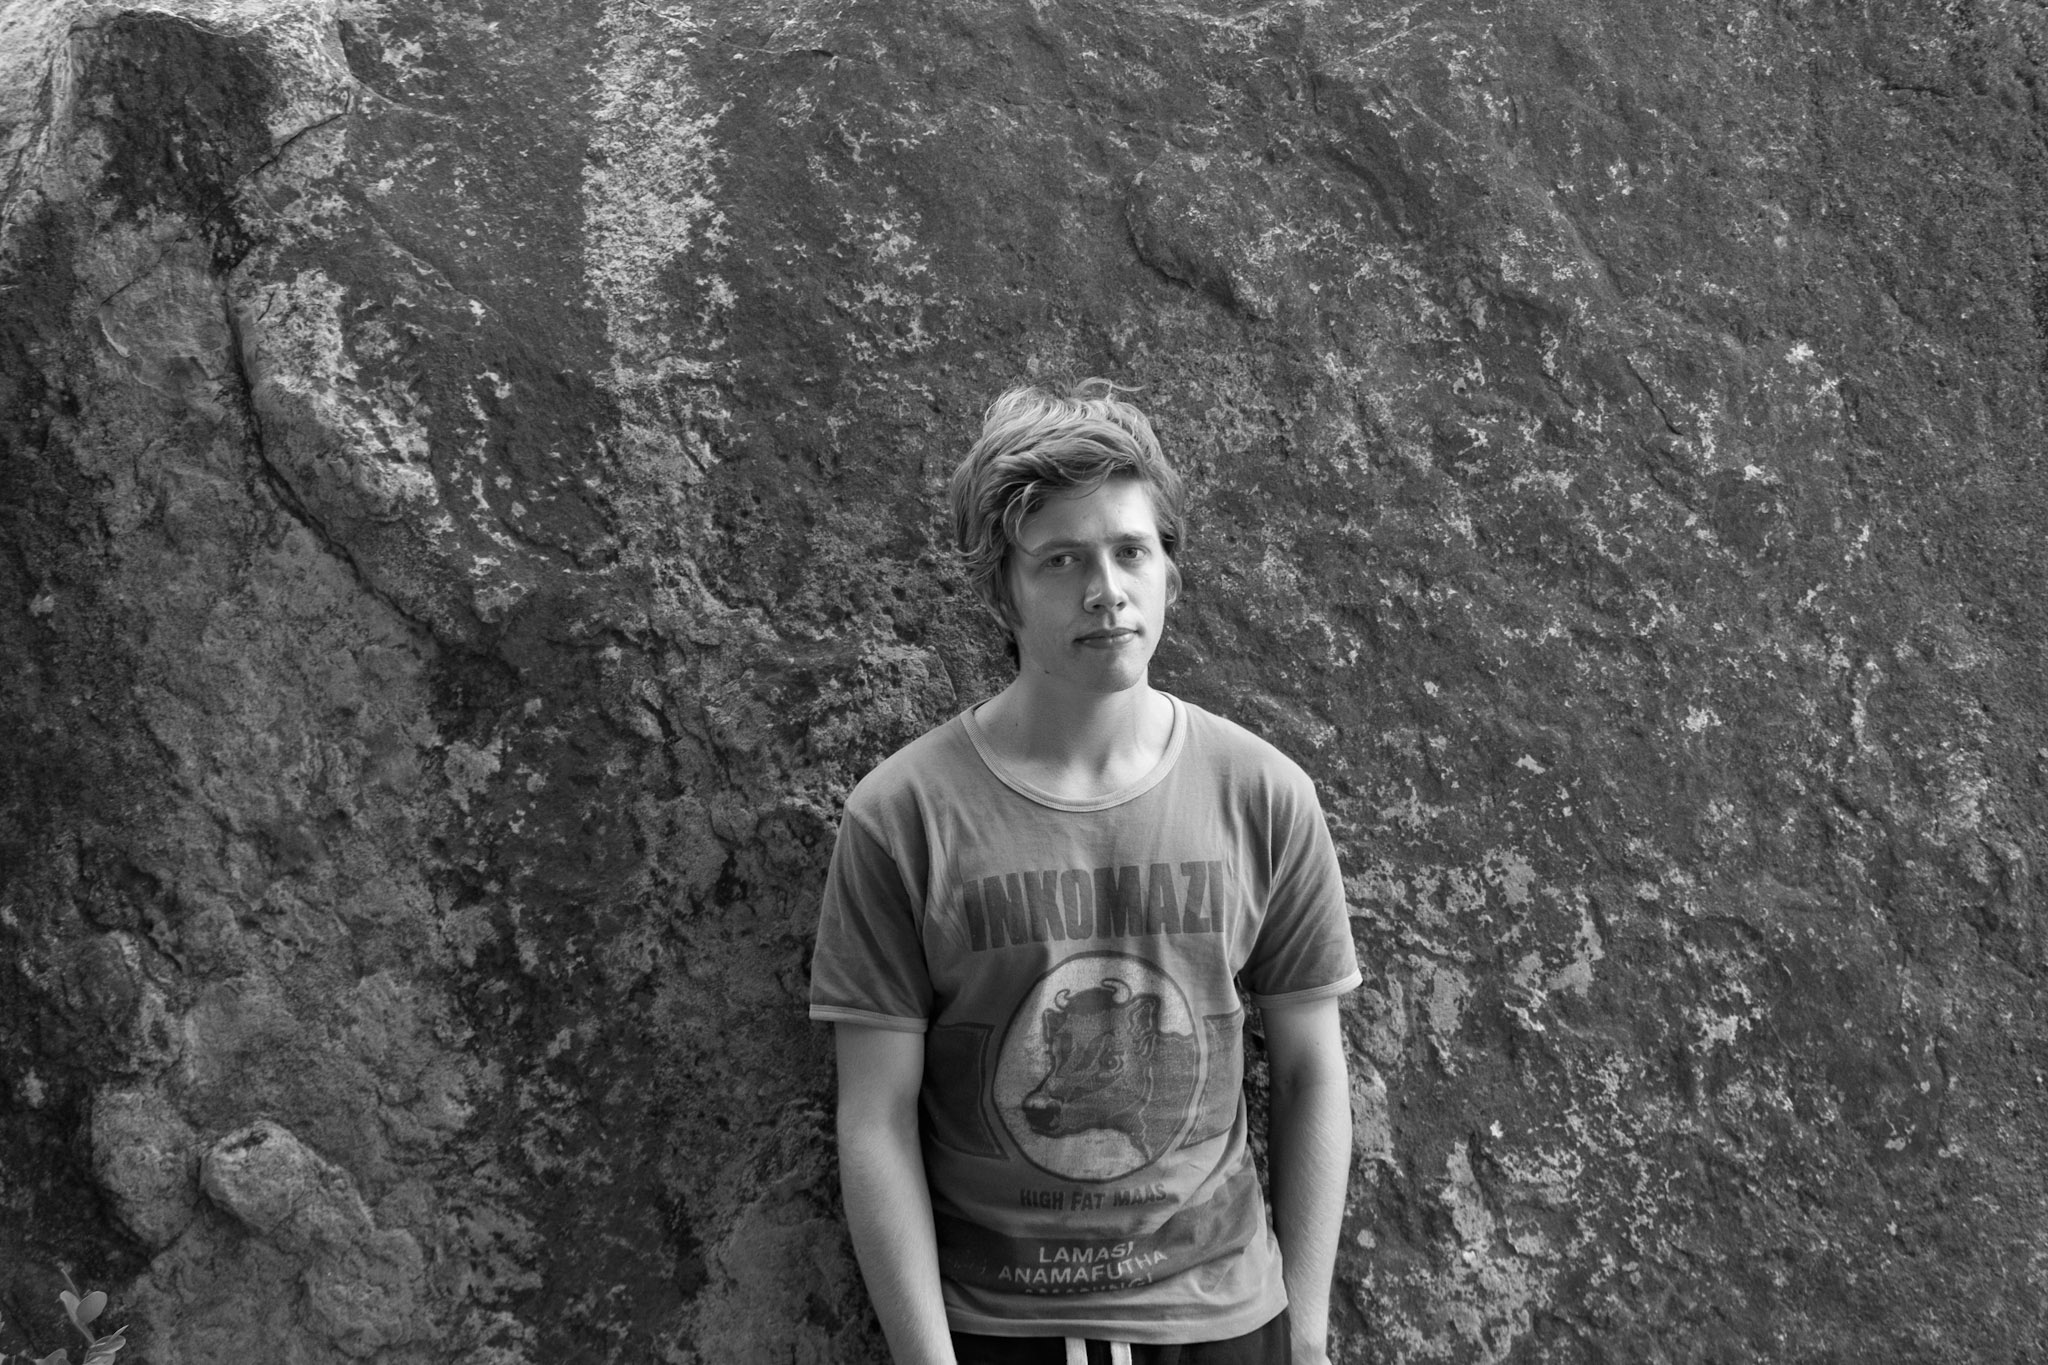
\includegraphics[width=0.7\textwidth]{../matthias.jpg}
		\caption{Matthias Harvey}
	\end{figure}
	\subsubsection{Interests}
	\begin{itemize}
		\item Computer graphics, artificial intelligence, game programming, simulations
		\item Mathematics
		\item Physics
		\item French - read, write. Speak - intermediate. Japanese – beginner
	\end{itemize}
	\subsubsection{Development and technology experience}
	
	\begin{tabular}{| l | c | r |}
		Java   & C\#     & F\#                          \\
		Git    & C++, NASM     & Haskell                     \\
		OpenGL & SQL     & HTML, CSS, JavaScript, PHP   \\
		Django & Unity3D & Python                     
	\end{tabular}

	\subsubsection{Past Experience \& Achievements}
	\begin{itemize}
		\item \textbf{Past Experience}
		\begin{itemize}
			\item Research Assistant for the SSFM Research Group
			\begin{itemize}
				\item University of Pretoria
				\item Assisting Prof. S. Gruner and Dr. N. Timm with research pertaining to Formal Methods - specifically 3-Valued Bounded Model Checking
			\end{itemize}
			\item Web Developer for Ms. Vreda Pieterse (Software engineering lecturer)
			\begin{itemize}
				\item University of Pretoria
				\item July 2014 - Present
			\end{itemize}
			\item Teaching Assistant
			\begin{itemize}
				\item University of Pretoria
				\item February 2015 - Present
			\end{itemize}
			
			\item Developer at Monkey \& River during 2015
			\begin{itemize}
				\item Pretoria
				\item Helped develop a web-based system (using ASP.NET MVC) to compare municipalities and districts in SA. See demo here: \href{http://salgabarometerdemo.org.za/RatingTool}{RatingTool}
				\item June 2015 - December 2015
			\end{itemize}
			
			\item Intern at Agnomen Design
			\begin{itemize}
				\item Agnomen Design. An indie-game studio based in Cape Town
				\item $ \pm 3 $ months experience during holidays since 2014
			\end{itemize}
		\end{itemize}
		
		\item \textbf{Achievements}
		\begin{itemize}
			\item High school science expo – silver at nationals (Electricity from cardboard)
			\item Completed an online course: Creative Coding (from Monash University) 2014
			\item Placed 5th at the national finals of the Standard Bank IT Challenge 2015
			\item Currently team leader of six selected students developing a web-based peer review system for the University of Pretoria
		\end{itemize}
	\end{itemize}
	
	\subsubsection{Non-technical Skills}
	
	\subsubsection{Motivation for Choosing Project}
	
	\cleardoublepage
	
	\subsection{Dillon Heins - 14035538}
	\subsubsection{Contact}
		\begin{itemize}
			\item \href{https://za.linkedin.com/in/dillon-heins-54275810a}{LinkedIn - Dillon Heins}
			\item \href{mailto:dillonheins@gmail.com}{dillonheins@gmail.com}	
		\end{itemize}
	\subsubsection{Photo}
		\begin{figure}[H]
			\centering
			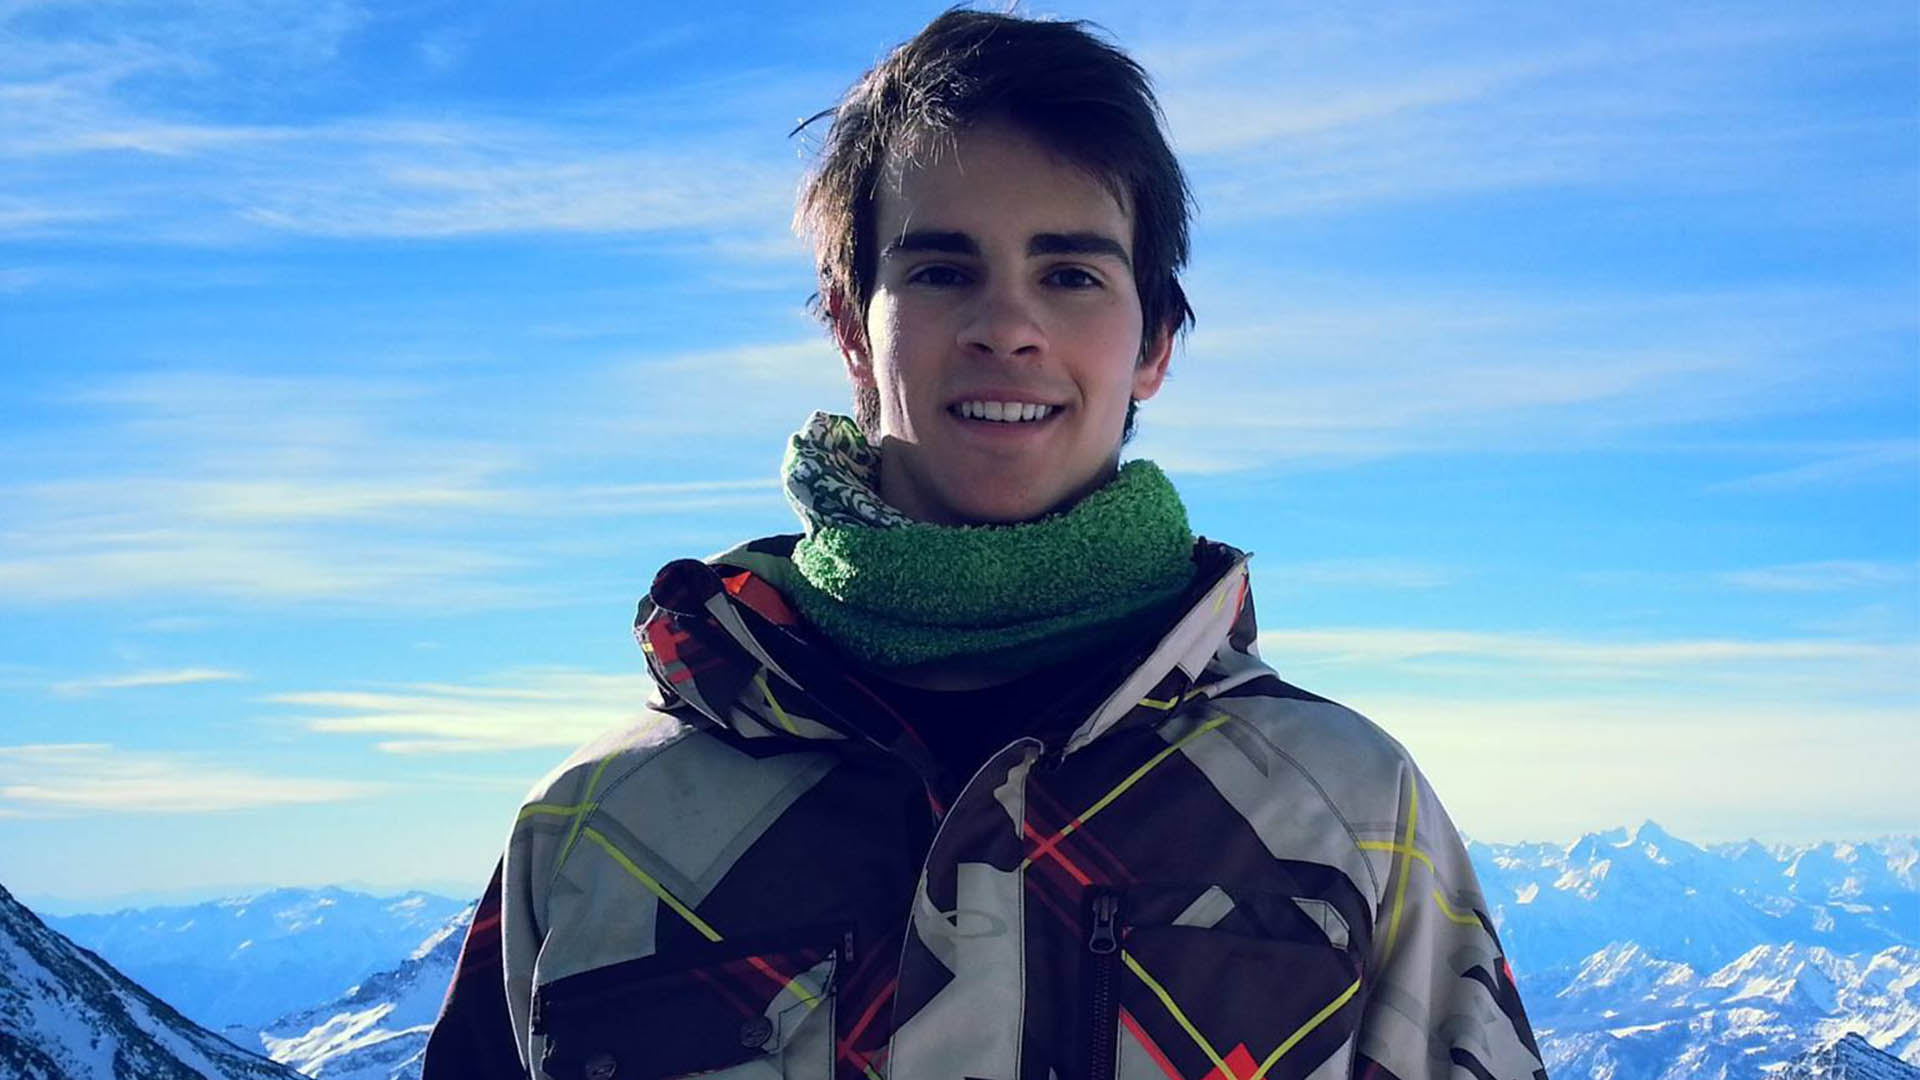
\includegraphics[width=0.7\textwidth]{../dillon.jpg}
			\caption{Dillon Heins}
		\end{figure}
	\subsubsection{Interests}
		\begin{itemize}
			\item Algorithms and data structures
			\item Computer networks
			\item Computer graphics
			\item Computer security
			\item Game development and design
		\end{itemize}
	\subsubsection{Technical Skills}
		\begin{itemize}
			\item Strong programming, algorithmic and data structure skills
			\item Proficient in the use of multimedia i.e. the combining of computer science, visual design and multimedia to create a complete and coherent product
			\item Adept in the learning and application of newly acquired skills
			\item Proficient in the programming and understanding of networked software
		\end{itemize}
	\subsubsection{Past Experience \& Achievements}
		\begin{itemize}
			\item \textbf{Past Experience}
			\begin{itemize}
				\item Web Developer for Ms. Vreda Pieterse (Software engineering lecturer)
				\begin{itemize}
					\item University of Pretoria
					\item July 2014 - Present
				\end{itemize}
				\item Teaching Assistant
				\begin{itemize}
					\item University of Pretoria
					\item February 2016 - Present
				\end{itemize}
			\end{itemize}
			
			\item \textbf{Achievements}
			\begin{itemize}
				\item
			\end{itemize}
		\end{itemize}
		
	\subsubsection{Non-technical Skills}
	\subsubsection{Motivation for Choosing Project}
	
	\newpage
	\subsection{Matthew Botha - 14214742}
		\subsubsection{Contact}
			\begin{itemize}
				\item \href{mailto:m.botha41@gmail.com}{m.botha41@gmail.com}
				\item Github: \href{https://github.com/MatthewBotha}{Matthew Botha}
			\end{itemize}
		\subsubsection{Photo}
		\begin{figure}[H]
			\centering
			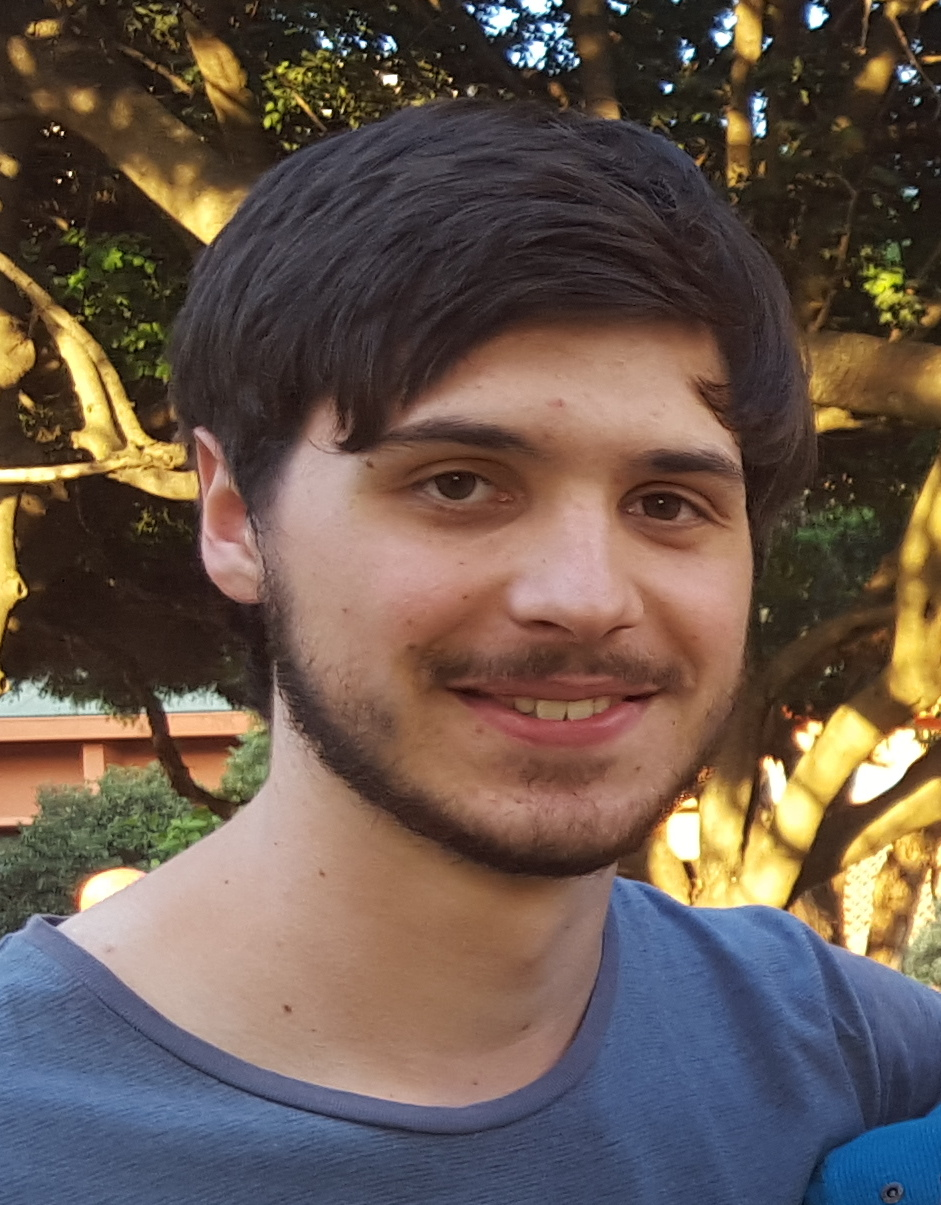
\includegraphics[width=250px]{../Matt.jpg}
			\caption{MatthewBotha}
		\end{figure}
		\subsubsection{Interests}
		\begin{itemize}
			\item Algorithms and data structures
			\item Computer security
			\item Computer architecture
			\item Computer networks
		\end{itemize}
		\subsubsection{Technical Skills}
		\begin{itemize}
			\item Programming Languages
			\begin{itemize}
				\item Java
				\item C
				\item C++
				\item C\#
				\item Pyhton
				\item Haskell
				\item x64 YASM Assembly 
			\end{itemize}
			\item Web developement
			\begin{itemize}
				\item HTML5
				\item PHP
				\item Django
				\item JavaScript
				\item ASP.NET
				\item Node.JS
				\item Bootstrap
			\end{itemize}
			\item Strong programming, algorithmic and data structure skills
			\item Adept in the learning and application of newly acquired skills
			\item Proficient in the programming and understanding of networked software
		\end{itemize}
		\subsubsection{Past Experience \& Achievements}
		\begin{itemize}
			\item \textbf{Past Experience}
			\begin{itemize}
				\item Web Developer for Ms. Vreda Pieterse (Software engineering lecturer)
				\begin{itemize}
					\item University of Pretoria
					\item July 2014 - Present
				\end{itemize}
				\item Teaching Assistant
				\begin{itemize}
					\item University of Pretoria
					\item August 2015 - Present
				\end{itemize}
			\end{itemize}
			
			\item \textbf{Achievements}
			\begin{itemize}
				\item Deputy Head Boy
				\begin{itemize}
					\item Hatfield Christian School
					\item 2013
				\end{itemize}
			\end{itemize}
		\end{itemize}
		
		\subsubsection{Non-technical Skills}
		\subsubsection{Motivation for Choosing Project}

\cleardoublepage
    
\section{Project Execution}

\end{document}
